\documentclass[10pt, a4paper]{amsart}

\usepackage{tikz}
\usetikzlibrary{decorations.pathreplacing}
\usepackage{graphicx}
\usepackage{float}
\usepackage[toc,page]{appendix}
\usepackage{listings}
\usepackage{physics}


\title[Periodic Structures]{Periodic Structures \\\hrulefill\small{ FYS3410: Problem Sheet 1 }\hrulefill}

\author{Candidate 33}

\date{\today}

\begin{document}

\maketitle

\section{One-Dimensional NaCl Crystal}

Figure \ref{fig:1DNaCl} shows a one-dimensional crystal of sodium chloride. The diatomic array is infinite and periodic. The atoms are equally space by a distance $a$.

\begin{figure}[ht]
	\centering
	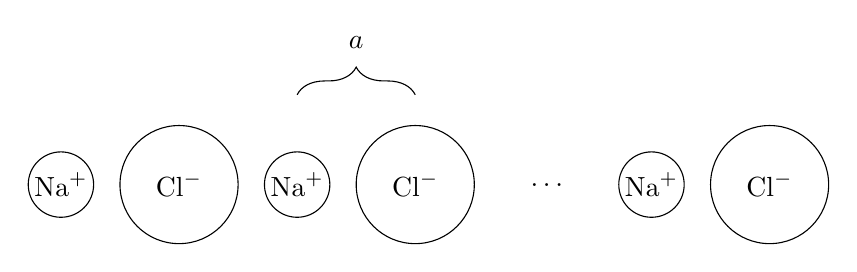
\begin{tikzpicture}
		\draw
		(1,1) node[circle, draw, inner sep=1pt]{$\text{Na}^+$}  
		(2.5,1) node[circle, draw, minimum size = 1.5cm]{$\text{Cl}^-$} 
		(4,1) node[circle, draw, inner sep=1pt]{$\text{Na}^+$}  
		(5.5,1) node[circle, draw, minimum size = 1.5cm]{$\text{Cl}^-$}
		(7,1)node[xshift = 0.2cm]{\dots}
		(8.5,1) node[circle, draw, inner sep=1pt]{$\text{Na}^+$}  
		(10,1) node[circle, draw, minimum size = 1.5cm]{$\text{Cl}^-$};
		\draw 
		[decorate,decoration={brace,amplitude=10pt,mirror,raise=4pt},yshift=0pt]
		(5.5,2) -- (4,2)  node [black,midway, yshift=0.8cm] {$a$};
	\end{tikzpicture}
	\caption{Infinite one-dimensional sodium chloride crystal.}
	\label{fig:1DNaCl}
\end{figure}

\subsection{Basis and unit cell}

The unit cell is the building block necessary to build the entire crystal. The unit cell one-dimensional crystal in figure \ref{fig:1DNaCl} is one diatomic set consisting of one sodium ion (Na$^+$) and one chlorine ion (Cl$^-$), spaced $a$ apart.

\begin{figure}[H]
	\centering
	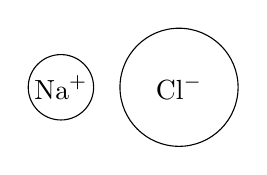
\begin{tikzpicture} 
	\draw	(1,1) node[circle, draw, inner sep=1pt]{$\text{Na}^+$}  
		 		(2.5,1) node[circle, draw, minimum size = 1.5cm]{$\text{Cl}^-$};
	\end{tikzpicture}
\end{figure}

A suitable lattice for this crystal would have lattice points placed $2a$ apart. The lattice vector would point to the right and have length of $2a$. The basis for the crystal is defined by the type, number and arrangement of atoms inside the unit cell. That is, one sodium ion and one chlorine ions placed horizontally in succession, $a$ apart.

\subsection{Derivation of Madelung's constant}

Madelung's constant if found by first computing the potential energy, or lattice energy of the crystal. This energy is computed from one the viewpoint of an initial ions as a sum of interactions with all other ions in the crystal. For this one-dimensional lattice, the interaction in one of the directions will be
\begin{equation}
U' = \sum_{n=1}^\infty -\frac{Qq_n}{r},
\end{equation}
where $q$ is the charge of the starting ion and $q_i$ the charge of some other ion in the lattice. The charges of the ions are the same, but the sign of the product will change. Moreover, the distance to a particular ion is $r=na$. This yields
\begin{equation}
U' = \sum_{n=1}^\infty -\frac{q^2(-1)^n}{na} = -\frac{q^2}{a}\sum_{n=1}^\infty \frac{(-1)^n}{n}.
\end{equation}
To include the other direction as well, one needs simply to multiply this by $2$
\begin{equation}
U = -\frac{q^2}{a} 2\sum_{n=1}^\infty \frac{(-1)^n}{n}.
\end{equation}
If
\begin{equation}
U_\alpha = -\frac{q^2}{a}\alpha,
\end{equation}
then Madelung's constant is
\begin{equation}
\alpha = 2\sum_{n=1}^\infty \frac{(-1)^n}{n}.
\end{equation}
This sum converges towards $2\ln(2)= 1.38629$, which means that the crystal is stable.

\subsection{Madelung's constant for a finite crystal}

\begin{figure}
	\centering
	\includegraphics[width=0.8\textwidth]{./figures/madelung.png}
	\caption{Convergence of Madelung's constant}
	\label{fig:madelung}
\end{figure}

Figure \ref{fig:madelung} shows a computation of Madelung's constant for different crystal sizes $N \in (1, 50)$. The convergence of the constant is apparent. The script used to generate this plot can be found in appendix \ref{app:madelung}.

\subsection{Repulsive and attractive forces}

\begin{figure}
	\centering
	\includegraphics[width=0.8\textwidth]{./figures/forces.png}
	\caption{Equilibrium of attractive and repulsive forces gives the distance between ions. A larger crystal has a higher lattice constant.}
	\label{fig:forces}
\end{figure}

The general condition related to the repulsive and attractive force balance that determines the realisation of a crystal is that the energy should be minimised. The equilibrium lattice constant can be computed numerically. The result of such a simulation is portrayed in figure \ref{fig:forces}. One can see that as the crystal is increasing in size, it becomes more stable and the lattice constant decreases. There is a clear convergence in this situation as well. The script that produces this plot can be found in appendix \ref{app:forces}.


\section{Reciprocal space in triclinic crystal}

\begin{figure}
	\centering
	\includegraphics[width = 0.6\textwidth]{./figures/problem4.png}
	\caption{Specific planes in a triclinic crystal.}
	\label{fig:triclinic}
\end{figure}

\subsection{Miller indices}

Figure \ref{fig:triclinic} shows a triclinic crystal with a set of lattice vectors $\vb{a}_1$, $\vb{a}_2$ and $\vb{a}_3$\footnote{$\vb{a}_3$ is directed toward the reader.}. The Miller indices for the planes in figure \ref{fig:triclinic} can be found in table \ref{tab:miller}. The Miller indices are found by the reciprocal intercepts
\begin{equation}
(\text{hkl}) = \left(\frac{1}{x_1}\frac{1}{x_2}\frac{1}{x_3}\right).
\end{equation}
When one are using Miller indices the planes are often referred to as $($hkl$)$ planes.

\begin{table}
	\centering
	\caption{Miller indices for planes in figure \ref{fig:triclinic}}
	\label{tab:miller}
	\begin{tabular}{lr} 
	No. & Miller \\ \hline
	1 	& (020) \\
	2	& (120) \\
	3 	& (010) \\
	4	& (210) \\
	5	& (200) \\
	6 	& (100) \\ \hline
	\end{tabular}
\end{table}

\begin{appendices}

\section{Script for Madelung's constant}
\label{app:madelung}
\lstinputlisting[language=python, showstringspaces=false]{./scripts/madelung.py}

\section{Script for simulation of Repulsive and Attractive forces}
\label{app:forces}
\lstinputlisting[language=python, showstringspaces=false]{./scripts/energyeqm.py}

\end{appendices}

\end{document}